\chapter{Working with Modules: Using Other People’s Code}

\section{Introduction: Real-Life Hook}

Imagine building a house.

Do you:
\begin{itemize}
    \item Make your own bricks?
    \item Make your own doors?
\end{itemize}

No.

You use:
\begin{itemize}
    \item Ready-made bricks
    \item Ready-made tools
\end{itemize}

In programming, these ready-made tools are called \textbf{Modules}.

\section{What Is a Module?}

\begin{definition}{Module}
A module is a file that contains \textbf{ready-made code} such as functions, variables, and classes.
\end{definition}

Modules help programmers:
\begin{itemize}
    \item Save time
    \item Avoid mistakes
    \item Write clean programs
\end{itemize}

\section{Why Modules Are Important}

Without modules:
\begin{itemize}
    \item Programs become very long
    \item Code is repeated again and again
\end{itemize}

With modules:
\begin{itemize}
    \item Programs become short
    \item Code is organized
\end{itemize}

\section{Types of Modules}

\begin{itemize}
    \item Built-in modules
    \item User-defined modules
    \item External modules
\end{itemize}

\section{Built-in Modules}

Python comes with many built-in modules.

Examples:
\begin{itemize}
    \item \texttt{math}
    \item \texttt{random}
    \item \texttt{datetime}
\end{itemize}

\subsection{Using the Math Module}

\begin{verbatim}
import math
print(math.sqrt(16))
\end{verbatim}

\textbf{Output:}
\begin{verbatim}
4.0
\end{verbatim}

\subsection{Using Random Module}

\begin{verbatim}
import random
print(random.randint(1, 6))
\end{verbatim}

Used in:
\begin{itemize}
    \item Games
    \item Simulations
\end{itemize}

\section{Different Ways to Import Modules}

\subsection{Import Entire Module}

\begin{verbatim}
import math
\end{verbatim}

\subsection{Import Specific Items}

\begin{verbatim}
from math import sqrt
print(sqrt(25))
\end{verbatim}

\subsection{Using Alias}

\begin{verbatim}
import math as m
print(m.pi)
\end{verbatim}

\section{User-Defined Modules}

You can create your own module.

\textbf{Step 1: Create file \texttt{tools.py}}

\begin{verbatim}
def add(a, b):
    return a + b

def subtract(a, b):
    return a - b
\end{verbatim}

\textbf{Step 2: Use the module}

\begin{verbatim}
import tools
print(tools.add(5, 3))
\end{verbatim}

\section{Real-Life Example: Calculator Toolkit}

Instead of writing calculator code again and again:
\begin{itemize}
    \item Write it once
    \item Use it everywhere
\end{itemize}

\section{Mini-Project: Dice Game Using Modules}

\begin{verbatim}
import random

print("Rolling dice...")
print(random.randint(1, 6))
\end{verbatim}

Students learn:
\begin{itemize}
    \item Code reuse
    \item Clean design
\end{itemize}

\section{Finding Modules}

Python module library includes:
\begin{itemize}
    \item Math functions
    \item Date and time
    \item File handling
\end{itemize}

(Advanced modules are introduced later.)

\section{Diagram: Module Usage Flow}

\begin{center}
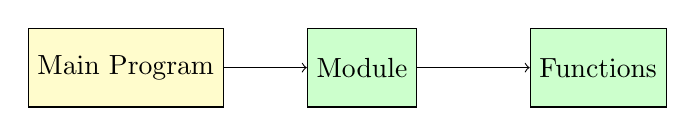
\begin{tikzpicture}[node distance=3cm]
\node (prog) [draw, rectangle, fill=yellow!20, minimum height=1cm] {Main Program};
\node (module) [draw, rectangle, fill=green!20, right of=prog, minimum height=1cm] {Module};
\node (func) [draw, rectangle, fill=green!20, right of=module, minimum height=1cm] {Functions};

\draw[->] (prog) -- (module);
\draw[->] (module) -- (func);
\end{tikzpicture}
\end{center}

\section{Best Practices}

\begin{itemize}
    \item Use modules to reduce code duplication
    \item Use clear module names
    \item Import only what you need
\end{itemize}

\section{Key Concepts}

\begin{itemize}
    \item Modules contain reusable code
    \item Built-in modules save time
    \item User-defined modules organize programs
    \item Import styles affect readability
\end{itemize}

\section{Common Beginner Mistakes}

\begin{itemize}
    \item Forgetting module name
    \item Naming file same as module
    \item Importing unnecessary modules
\end{itemize}

\section{End-of-Chapter Exercises}

\subsection{Very Short Questions}

\begin{enumerate}
    \item What is a module?
    \item Name two built-in modules.
    \item What does \texttt{import} do?
\end{enumerate}

\subsection{Short Answer Questions}

\begin{enumerate}
    \item Explain module using real-life example.
    \item Difference between built-in and user-defined modules.
    \item What is alias in module import?
\end{enumerate}

\subsection{Activity-Based Exercises}

\begin{enumerate}
    \item Create your own math module.
    \item Use \texttt{random} to create a number guessing game.
    \item Modify a program to use modules instead of repeated code.
\end{enumerate}

\section{Teacher Notes}

\marginnote{
\textbf{Learning Objectives}
\begin{itemize}
    \item Students understand module concept
    \item Students use built-in modules
    \item Students create user-defined modules
\end{itemize}

\textbf{Teaching Tips}
\begin{itemize}
    \item Compare modules with toolboxes
    \item Show reduction of code length
    \item Encourage reuse mindset
\end{itemize}

\textbf{Assessment}
\begin{itemize}
    \item Proper module usage
    \item Correct import statements
\end{itemize}
}